\documentclass[xcolor={dvipsnames,usenames}]{beamer}
%\documentclass[xcolor={dvipsnames,usenames},handout]{beamer} % use this to compile w/o pauses
\mode<presentation>
{
\usetheme{madrid}
\usecolortheme{default}
\setbeamertemplate{itemize items}[default]
\setbeamertemplate{enumerate items}[default]
\setbeamercovered{transparent}
\usefonttheme[onlymath]{serif}
}


\usepackage{microtype}

%\usepackage{hyperref}
%\hypersetup{colorlinks=true, urlcolor=Blue, citecolor=Green, linkcolor=BrickRed, breaklinks, unicode}

\usepackage[nocompress]{cite}
\usepackage{amsmath,mathtools,stmaryrd}
\usepackage{enumerate}
\usepackage{latexsym,amsmath}
\usepackage{amssymb,stmaryrd}
\usepackage{euscript}
\usepackage{algorithm,algorithmicx}
\usepackage[noend]{algpseudocode}
\renewcommand{\algorithmicrequire}{\textbf{Requirement:}}

\usepackage{mathtools} % for \coloneqq

\usepackage{graphicx}
\usepackage{epstopdf}
\usepackage{subcaption}
\graphicspath{{./fig/}}


\title{Approximate Minimum-Weight Partial Matching under~Translation}
\author[Allen Xiao]
{
	Pankaj~Agarwal \inst{1} \and
	Haim~Kaplan \inst{2} \and
	Geva~Kipper \inst{2} \and
	Wolfgang~Mulzer \inst{3} \and
	G{\"u}nter~Rote \inst{3} \and
	Micha~Sharir \inst{2} \and
	Allen~Xiao \inst{1}
}
\institute[ISAAC 2018]
{
	\inst{1} Duke University \and
	\inst{2} Tel Aviv University \and
	\inst{3} Freie Universit{\"a}t Berlin
}
\date{December 2018}

% tweak wd=X\paperwidth to modify the footer dimensions in the madrid theme
\makeatletter
\setbeamertemplate{footline}{
  \leavevmode%
  \hbox{%
  \begin{beamercolorbox}[wd=.25\paperwidth,ht=2.25ex,dp=1ex,center]{author in head/foot}%
    \usebeamerfont{author in head/foot}\insertshortauthor\expandafter\ifblank\expandafter{\beamer@shortinstitute}{}{~~(\insertshortinstitute)}
  \end{beamercolorbox}%
  \begin{beamercolorbox}[wd=.55\paperwidth,ht=2.25ex,dp=1ex,center]{title in head/foot}%
    \usebeamerfont{title in head/foot}\insertshorttitle
  \end{beamercolorbox}%
  \begin{beamercolorbox}[wd=.2\paperwidth,ht=2.25ex,dp=1ex,right]{date in head/foot}%
    \usebeamerfont{date in head/foot}\insertshortdate{}\hspace*{2em}
    \insertframenumber/\inserttotalframenumber \hspace*{2ex}
  \end{beamercolorbox}}%
  \vskip0pt%
}
\makeatother


% make tables less packed
\renewcommand{\arraystretch}{1.5}
% get rid of caption labels
%\setbeamertemplate{caption}{\raggedright\insertcaption\par}
%\captionsetup[subfigure]{labelformat=empty}
% set beamer highlight color (alert)
\setbeamercolor{alerted text}{fg=BrickRed}

\newcommand{\mycite}[1]{{\color{LimeGreen}\lbrack #1\rbrack}}
\newcommand{\etal}{\textit{et~al.}}
\newcommand{\softO}{\widetilde{O}}
\newcommand{\reals}{\mathbb{R}}
\newcommand{\ints}{\mathbb{N}}
\newcommand\nats{\mathbb{N}}
\newcommand{\eps}{\varepsilon}
\DeclareMathOperator{\polylog}{polylog}
\DeclareMathOperator{\poly}{poly}
\newcommand{\flr}[1]{{\lfloor #1\rfloor}}
\DeclareMathOperator*{\argmax}{arg\,max}
\DeclareMathOperator*{\argmin}{arg\,min}
\DeclareMathOperator{\Vor}{Vor}
\DeclareMathOperator{\VorRegion}{VorRegion}

\def\abs#1{\mathopen| #1 \mathclose|}		% use instead of $|x|$
\def\norm#1{\mathopen\| #1 \mathclose\|}	% use instead of $\|x\|$

\DeclareMathOperator{\cost}{cost}
\newcommand{\tsupply}{\lambda}
\newcommand{\fsupply}{\phi}

\newcommand{\A}{{\color{red}A}}
\newcommand{\B}{{\color{blue}B}}
\newcommand{\M}{\EuScript{M}}
\newcommand{\tildeM}{\widetilde{\EuScript{M}}}
\newcommand{\X}{\EuScript{X}}

\def\EMPH#1{\textcolor{BrickRed}{{\emph{#1}}}}



\begin{document}


\begin{frame}
\maketitle
\end{frame}


% outline
% problem demonstration, refer to static problem
% formal statements: 
%	l_p cost function, 
%	P1: find the optimal translation, and 
%	P2: complexity (no. faces) of the minimization diagram
% 	studied previously for p=2 (rms), but even for p=2 whether M is polynomial is open
%	best bound for p=2: O(n^2m^3.5 (e\ln m + e)^m)
% results:
% 	P2: polynomial complexity approximate diagram
%	P1: polytime approximation algorithm after constructing approx. diagram
% outline for approx diagram:
%	Lipschitz continuity for cost() under any l_p cost
%	given that, point-to-point translations (Cabello et al.) are a constant approx.
%	tile cells with an \eps-grid (also Cabello et al.) to improve to (1+\eps)
%	reduced set of centers: greedy disk eating
% algorithm for P1: apply a stationary k-matching algorithm to each center
% state Lipschitz property (calculation?)
% point-to-point translations and constant approx
% eps-grid tiling
% smaller set of centers


%SECTION: pmt

% gentle example + equation
\begin{frame}{Example}
% point sets A and B of size m, n respectively
% allowed to translate A --> A+t
% minimum-cost k-matching between A+t and B
% what's the best translation?
\begin{figure}
\begin{center}
\includegraphics<1>[width=\textwidth,page=1]{pmt_example}%
\includegraphics<2>[width=\textwidth,page=2]{pmt_example}%
\includegraphics<3>[width=\textwidth,page=3]{pmt_example}%
\includegraphics<4>[width=\textwidth,page=4]{pmt_example}%
\includegraphics<5>[width=\textwidth,page=5]{pmt_example}%
\includegraphics<6>[width=\textwidth,page=6]{pmt_example}%
\includegraphics<7->[width=\textwidth,page=7]{pmt_example}%
\end{center}
\end{figure}
\end{frame}

% introduce cost function
\begin{frame}{Cost function}
% equation
% static problem (t fixed) has polytime algorithms, e.g. Hungarian algorithm [RT]
\begin{itemize}
\item For $k$-matching $M$ and translation $t$, define the \EMPH{$L_p$-cost}:
	\begin{equation*}
	\cost(M, t) \coloneqq \left[\frac{1}{k}\sum_{(a, b) \in M}\norm{a+t-b}^p\right]^{1/p}
	\end{equation*}
\pause
\item $p = 2$: root-mean-squared cost
\pause
\item For fixed $t$, minimum $M$ computable in $\poly(k, m, n)$ time, \\
	e.g. by Hungarian algorithm.
\end{itemize}
\end{frame}

% minimization diagram M
\begin{frame}{Minimization diagram $\M$}
% function over t for each k matching
% cost*(t): the lower envelope
% vertical projection subdivides the plane
\begin{equation*}
\cost^*(t) \coloneqq \min_{\text{$k$-matching $M$}} \cost(M, t)
\end{equation*}
\begin{figure}
\begin{center}
\includegraphics<1>[width=0.6\textwidth,page=1]{lower_env}%
\includegraphics<2>[width=0.6\textwidth,page=2]{lower_env}%
\includegraphics<3>[width=0.6\textwidth,page=3]{lower_env}%
\includegraphics<4>[width=0.6\textwidth,page=4]{lower_env}%
\includegraphics<5>[width=0.6\textwidth,page=5]{lower_env}%
\includegraphics<6>[width=0.6\textwidth,page=6]{lower_env}%
\includegraphics<7>[width=0.6\textwidth,page=7]{lower_env}%
\includegraphics<8->[width=0.6\textwidth,page=8]{lower_env}%
\end{center}
\end{figure}
\end{frame}

% main questions
\begin{frame}{Questions and prior results}
% what is the combinatorial complexity of M?
%	p=2: ben-avraham et al bound
%	rote: line intersects poly(n) cells
% can we compute t*, the minimum point of cost*(t)?
%	existing algorithm: traverse all cells of M (given point, find boundaries)
\begin{enumerate}
\item {\large What is the \EMPH{combinatorial complexity of $\M$}? Is it polynomial?}
	\begin{itemize}
	\item \mycite{Rote 10}: for $p=2$ and $k=m$, \\
		a line crosses at most $m(n-m) + 1$ cells 
	\item \mycite{Ben-Avraham~{\etal} 14}: for $p=2$ and $k=m$, \\
		$O(n^2 m^{3.5}(e \ln m + e)^m)$ 
	\end{itemize}
\item {\large How quickly can we \EMPH{compute $t^*$}, a global minimum of $\cost^*(t)$?}
	\begin{itemize}
	\item Explore $\M$, use static algorithm within cells.
	\end{itemize}
\end{enumerate}
\end{frame}

% approximate diagram
\begin{frame}{Approximating $\M$}
\begin{figure}
\begin{center}
\includegraphics<1>[width=0.8\textwidth,page=1]{approx_diagram}%
\includegraphics<2>[width=0.8\textwidth,page=2]{approx_diagram}%
\includegraphics<3>[width=0.8\textwidth,page=3]{approx_diagram}%
\includegraphics<4>[width=0.8\textwidth,page=4]{approx_diagram}%
\includegraphics<5>[width=0.8\textwidth,page=5]{approx_diagram}%
\includegraphics<6->[width=0.8\textwidth,page=6]{approx_diagram}%
\end{center}
\end{figure}
\end{frame}

% take away: approximation gives polynomial solutions to both
\begin{frame}{Our results (approximation helps)}
% what is the combinatorial complexity of M?
%	we can construct an /approximate/ diagram ~M with polynomial size
%	each cell \tau of ~M has an associated matching M_\tau, \cost(M_\tau) approximates \cost*(t) for all t \in \tau
% can we compute t*, the minimum point of cost*(t)?
%	polytime algorithm by traversing all cells of ~M
\begin{enumerate}
\item {\large What is the \EMPH{combinatorial complexity of $\M$}? Is it polynomial?}
	\begin{theorem}
	In $\poly(k, m, n, \eps^{-1})$ time, can construct a $(1+\eps)$
	\EMPH{approximate diagram} $\tildeM$ of complexity
	$O((mn/k)\eps^{-2}\log\eps^{-1})$.
	\end{theorem}
\item {\large How quickly can we \EMPH{compute $t^*$}, a global minimum of $\cost^*(t)$?}
	\begin{theorem}
	In $\poly(k, m, n, \eps^{-1})$ time, can compute a $(1+\eps)$ \\
	\EMPH{approximation to $\cost^*(t^*)$} by exploring the cells of $\tildeM$.
	\end{theorem}
\end{enumerate}
\end{frame}

% Lipschitz property --> point-to-point translations
\begin{frame}{Point-to-point translations \mycite{Cabello~{\etal} 08}}
% originally used by Cabello for for EMD under translations
% punchline: Vor(T) is constant approximate diagram!
\begin{itemize}
\item \EMPH{Point-to-point translations}: $T \coloneqq \{t_{ba} = (b - a) \mid a \in A, b \in B\}$
\begin{figure}
\begin{center}
\includegraphics<1>[width=0.6\textwidth,page=1]{point-to-point}%
\includegraphics<2>[width=0.6\textwidth,page=2]{point-to-point}%
\includegraphics<3>[width=0.6\textwidth,page=3]{point-to-point}%
\includegraphics<4>[width=0.6\textwidth,page=4]{point-to-point}%
\includegraphics<5->[width=0.6\textwidth,page=5]{point-to-point}%
\end{center}
\end{figure}
\item<6-> Claim: Let $\tildeM$ be $\Vor(T)$, with each $\VorRegion(t_{ba})$ assigned the optimal $k$-matching at $t_{ba}$.
	Then, $\tildeM$ is a $O(1)$-approximate diagram.
\end{itemize}
\end{frame}

% key idea: L_p cost has Lipschitz property
\begin{frame}{Lipschitz continuity for $L_p$-cost}
% ``moving a short distance cannot increase \cost*(t) by much''
\begin{equation*}
\cost(M, t) \coloneqq \left[\frac{1}{k}\sum_{(a, b) \in M}\norm{a+t-b}^p\right]^{1/p}
\end{equation*}
\begin{lemma}[Lipschitz condition]
Given $t, \Delta \in \reals^2$, let $M_t$ be the optimal $k$-matching at $t$. \\
Then $\cost(M_t, t+\Delta) \leq \cost^*(t) + \norm{\Delta}$.
\end{lemma}
%\begin{corollary}[Lipschitz condition]
%Let $t_1, t_2 \in \reals^2$, then $\cost^*(t_2) \leq \cost^*(t_1) + \norm{t_2 - t_1}$.
%\end{corollary}
\end{frame}

% point-to-point translations proof
\begin{frame}{Proof of approximation for $T$}
% by massaging the cost function: there is a point of T relatively close to every t
\begin{itemize}
\item Claim: $\tildeM$ is an $O(1)$-approximate diagram.
\item Given $t \in \reals^2$, let $t_0$ be its nearest neighbor in $T$,\\
	and $M_{t_0}$ the optimal matching at $t_0$.
\end{itemize}
\begin{equation*}
\begin{aligned}
\onslide<1->{\cost^*(t) &= \min_{\text{$k$-matching $M$}} \left[\frac{1}{k}\sum_{(a, b) \in M}\norm{a+t-b}^p\right]^{1/p} \\}
	\onslide<2->{&= \min_{\text{$k$-matching $M$}} \left[\frac{1}{k}\sum_{(a, b) \in M}\norm{t - \alert{t_{ba}}}^p\right]^{1/p} \\}
	\onslide<3->{&\geq \min_{\text{$k$-matching $M$}} \left[\frac{1}{k}\sum_{(a, b) \in M}\norm{t - \alert{t_0}}^p\right]^{1/p} \\}
	\onslide<4->{&= \norm{t - t_0}}
\end{aligned}
\end{equation*}
\end{frame}

% constant approximate diagram
\begin{frame}{Proof of approximation for $T$ (cont.)}
% Lipschitz + point-to-point -->
% Vor(T) is a constant approximate diagram!
\begin{itemize}
\item Claim: $\tildeM$ is an $O(1)$-approximate diagram.
\item Given $t \in \reals^2$, let $t_0$ be its nearest neighbor in $T$,\\
	and $M_{t_0}$ the optimal matching at $t_0$.
\item $\norm{t - t_0} \leq \cost^*(t)$
\end{itemize}
\begin{equation*}
\begin{aligned}
\onslide<2->{\cost(M_{t_0}, t) &\leq \cost^*(t_0) + \norm{t - t_0} & \text{(Lipschitz cond.)}\\}
	\onslide<3->{&\leq \cost^*(t) + 2\norm{t - t_0} & \text{(Lipschitz cond.)}\\}
	\onslide<4->{&\leq \cost^*(t) + 2\cost^*(t) \\}
	\onslide<5->{&= 3\cost^*(t)}
\end{aligned}
\end{equation*}
\end{frame}

% constant --> (1+eps)
\begin{frame}{$O(1)$ $\rightarrow$ $(1+\eps)$ approximation}
% grid cell width 2^i cost^*(t_0)
% resulting complexity is O((mn/\eps^2) \log(1/\eps))
\begin{figure}
\begin{center}
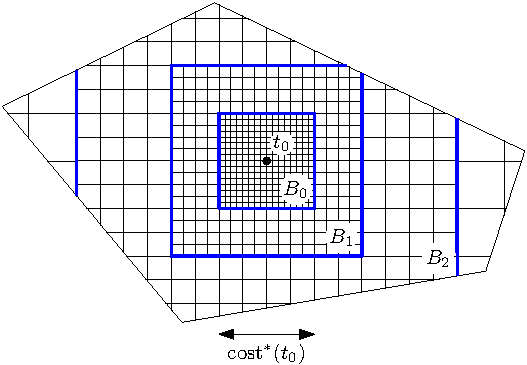
\includegraphics[width=0.5\textwidth,page=1]{nested-grid-crop}%
\end{center}
\end{figure}
\begin{itemize}
\item $(1+\eps)$ approximate diagram of size
	$O(\abs{T}\eps^{-2}\log\eps^{-1}) = O((mn)\eps^{-2}\log\eps^{-1})$
\end{itemize}
\pause
\begin{theorem}
In $\poly(k, m, n, \eps^{-1})$ time, can construct a $(1+\eps)$ approximate
diagram $\tildeM$ of complexity $O(\alert{(mn/k)}\eps^{-2}\log\eps^{-1})$.
\end{theorem}
\end{frame}

% compressing ~M further
\begin{frame}{Compressing $\tildeM$}
% any O(1) approx is fine to apply the constant --> (1+eps) transformation
% cluster T? how to ensure cluster radius small wrt cost*(t)?
% here: reduce the size O(mn) to O(mn/k)
\begin{itemize}
\item Reduce size from $O(mn) \rightarrow O(mn/k)$.
\item Any $O(1)$ approx. diagram is enough for the $(1+\eps)$ diagram.
\item \EMPH{Cluster the points of $T$}\ldots
	while keeping cluster radius small w.r.t. $\cost^*(t)$.
\end{itemize}
\end{frame}

% key idea: averaging argument
\begin{frame}{Averaging argument}
% look at the cost function again
% ``for matching M of cost \mu, there are \leq k/2 pairs with \norm{a-b} \geq 2\mu''
% add translation t --> M_t
% ``for matching M_t of cost \mu, there are \leq k/2 pairs with \norm{t - t_ab} \geq 2\mu''
\begin{equation*}
\cost^*(t) \coloneqq \min_{\text{$k$-matching $M$}} \left[\frac{1}{k}\sum_{(a, b) \in M}\norm{a+t-b}^p\right]^{1/p}
\end{equation*}
\begin{itemize}
\item At most $k/2$ pairs $(a, b) \in M_t$ have $\norm{a+t-b} \geq 2^{1/p}\cost^*(t)$.
\pause
\item At most $k/2$ pairs $(a, b) \in M_t$ have $\norm{t-\alert{t_{ab}}} \geq 2^{1/p}\cost^*(t)$.
\pause
\item \alert{At least} $k/2$ pairs $(a, b) \in M_t$ have $\norm{t-t_{ab}} \alert{\leq} 2^{1/p}\cost^*(t)$.
\end{itemize}
\end{frame}

% averaging argument picture
\begin{frame}{Averaging argument (cont.)}
% ``for matching M_t of cost \cost^*(t), there are \leq k/2 pairs with \norm{t - t_ab} \geq 2^{1/p}\cost^*(t)''
\begin{itemize}
\item \alert{At least} $k/2$ pairs $(a, b) \in M_t$ have $\norm{t-t_{ab}} \alert{\leq} 2^{1/p}\cost^*(t)$.
\end{itemize}
\begin{figure}
\begin{center}
\includegraphics<1>[width=0.6\textwidth,page=1]{ptp_in_disk}%
\includegraphics<2>[width=0.6\textwidth,page=2]{ptp_in_disk}%
\includegraphics<3->[width=0.6\textwidth,page=3]{ptp_in_disk}%
\end{center}
\end{figure}
\end{frame}

% greedy clustering by quorum clustering
\begin{frame}{Clustering $T$ greedily}
% inherit figure
% find the (approx.) smallest disk D_i containing at least k/2 points of T, center x_i, radius r_i
% remove covered points from T, and repeat
% 2-approx. algorithm: O(|T|\polylog n) by Carmi et al.
\begin{enumerate}
\item Let $D_i = B(x_i, r_i)$ be the smallest disk containing at least $k/2$ remaining points of $T$.
\item Remove from $T$ the points covered by $D_i$.
\item Repeat.
\end{enumerate}
%TODO replace above with figure?
\begin{itemize}
\pause
\item \EMPH{Quorum clustering}\\
	$2$-approx. algorithm in $O(\abs{T}\polylog n)$ time \mycite{Carmi~{\etal} 05}
\pause
\item $O(\abs{T}/k) = O(mn/k)$ clusters.
\end{itemize}
\end{frame}

% quorum clustering gives a constant approx
\begin{frame}{Greedy clustering proof of approximation}
% let X be the set of centers x_i, and ~M = Vor(X)
% proof by figure?
% for any translation t, consider disk D of radius 2^{1/p}\cost^*(t) centered at t
% D covers at least k/2 points of T
% let i^* be the first index where D_i^* covers a point of D \cap T
% since D_i^* is (approx) min-radius, r_i^* \leq 2* 2^{1/p}\cost^*(t)
% so, \norm{t - x_i^*} \leq 3*2^{1/p}\cost^*(t)
% as a NN, \norm{t - x_0} \leq 6\cost^*(t)
% apply the Lipschitz property --> Vor(X) is O(1)-approx diagram
% apply the grid refinement --> (1+\eps) approx diagram of size O((mn/k\eps^2)\log(1/\eps))
\begin{itemize}
\item Let $X$ be the set of centers $x_i$ from the greedy clustering,
	and $\tildeM = \Vor(X)$ with each $\VorRegion(x_i)$ assigned $M_{x_i}$.
\end{itemize}
\begin{figure}
\begin{center}
\includegraphics<1>[width=0.7\textwidth,page=1]{cluster_proof}%
\includegraphics<2>[width=0.7\textwidth,page=2]{cluster_proof}%
\includegraphics<3>[width=0.7\textwidth,page=3]{cluster_proof}%
\includegraphics<4>[width=0.7\textwidth,page=4]{cluster_proof}%
\includegraphics<5->[width=0.7\textwidth,page=5]{cluster_proof}%
\end{center}
\end{figure}
\end{frame}

% cont.
\begin{frame}{Greedy clustering proof of approximation}
\begin{figure}
\begin{center}
\includegraphics[width=0.7\textwidth,page=5]{cluster_proof}%
\end{center}
\end{figure}
\begin{itemize}
\item $\cost(M_{x_i}, t) \leq (1+6\cdot 2^{1/p}) \cost^*(t)$
\item Using grids, $(1+\eps)$ approx. diagram of size
	$O((mn/k) \eps^{-2}\log \eps^{-1})$.
\end{itemize}
\end{frame}

% lower bound on approx. diagram size when k is a constant fraction of m (m \leq n)
\begin{frame}{Lower bound: $O(mn/k)$ tight for large $k$}
% O(mn/k) = O(n)
% figure of [\sqrt{n}]^2 and [\sqrt{m}]^2 grid
% \Omega(n) translations where they are perfectly aligned with \geq k points in common (cost^*(t) = 0)
% at least \Omega(n) faces in any constant-approx diagram
\begin{itemize}
\item For $k = c\cdot\min(m, n)$, constant $c$:
\end{itemize}
\begin{figure}
\begin{center}
\includegraphics<1>[width=0.7\textwidth,page=1]{lower_bound_big_k}%
\includegraphics<2>[width=0.7\textwidth,page=2]{lower_bound_big_k}%
\includegraphics<3>[width=0.7\textwidth,page=3]{lower_bound_big_k}%
\includegraphics<4->[width=0.7\textwidth,page=4]{lower_bound_big_k}%
\end{center}
\end{figure}
\end{frame}

% open questions
\begin{frame}{Open questions}
% is the complexity of the exact minimization diagram polynomial? for p=2?
% approximate diagrams for rotations? rigid transforms?
\begin{enumerate}
\item Is the complexity of $\M$ polynomial, for any $p$?
\item Approximate diagrams for rotations? Rigid transforms?
\end{enumerate}
\end{frame}

% 20
%\begin{frame}
%\end{frame}

\begin{frame}{The End}
\begin{center}
	Thank you.
\end{center}
\end{frame}

%\begin{frame}[allowframebreaks]{Citations}
%\tiny
%\bibliography{ref}
%\bibliographystyle{alpha}
%\end{frame}


\end{document}
